
%%%%%%%%%%%%%%%%
%%%%%%%%%%%%%%%%

\section{Simple DEC analysis} \label{sec:bg_simple}


The following series of tutorials will reconstruct the ancestral ranges of the silversword alliance (Tribe {\it Madiinae}), a young and diverse clade of about 50 species \citep{Baldwin1991}.
Although silverswords are endemic to Hawaii, they are nested within a larger clade alongside tarweeds, which are native to the California coastline.
The size and age of the silversword clade, combined with our knowledge of Hawaiian island formation, makes it an ideal system to explore concepts in historical biogeography and phylogeny.
For further reading, consult: \citet{Carlquist1959, Baldwin1998}.
 
\begin{figure}[!ht]
\centering
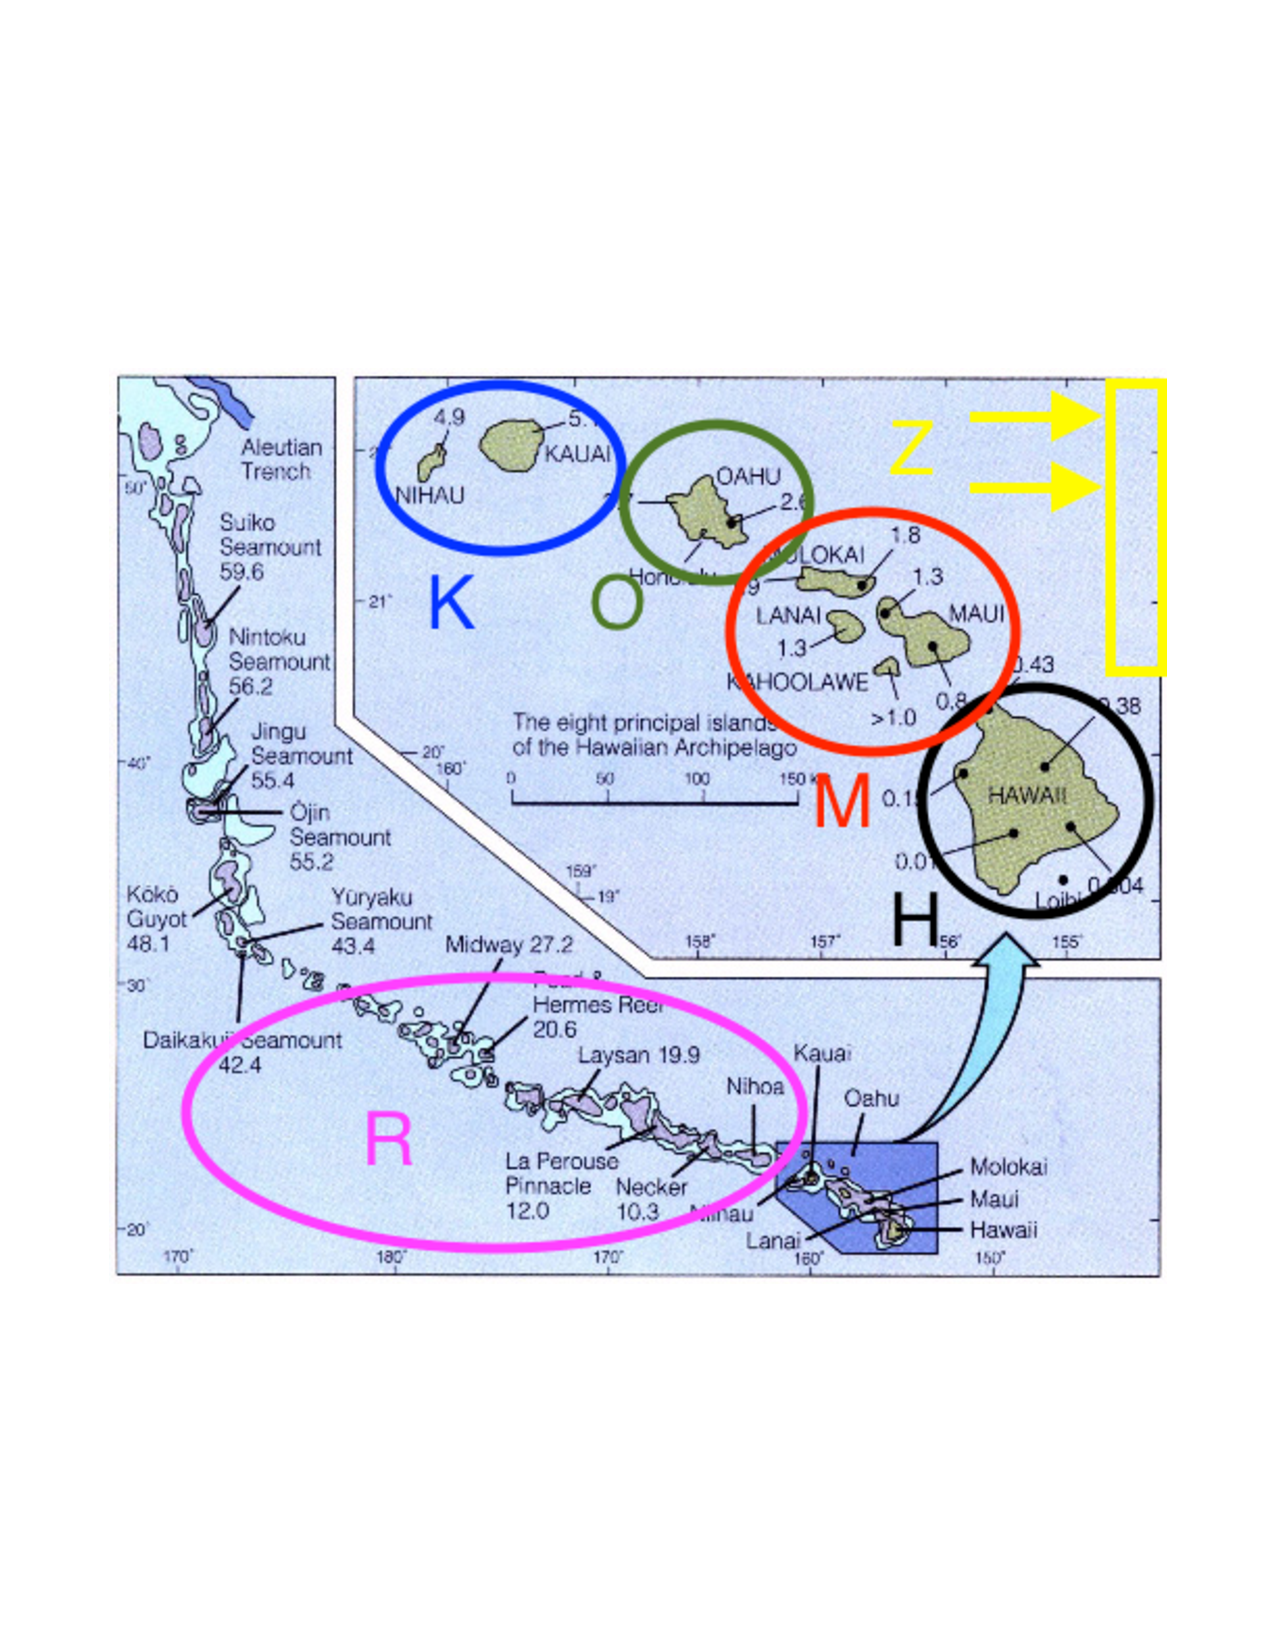
\includegraphics[width=0.6\textwidth]{figures/fig_hawaii_areas.pdf}
\caption{A beautiful figure of the discrete areas for tutorial. Six areas are shown: Kauai and Niihau (K); Oahu (O); Maui-Nui, Lanai, and Molokai (M); Hawaii (H); the remaining Hawaiian islands (R); and the North American mainland (Z).}
\label{fig:hawaii_areas}
\end{figure}
 
For this tutorial we'll focus entirely on the silversword alliance and the modern Hawaiian archipelago.
To begin, we'll use just four areas, K, O, M, and H, and include areas R and Z in later analyses (Fig \ref{fig:hawaii_areas}).

\begin{table}[!ht]
\centering
\begin{tabular}{llcc}
Range & Areas & Size & State \\ \hline
$\emptyset$ & 0000 & 0 & 0 \\
K    & 1000 & 1 & 1 \\
O    & 0100 & 1 & 2 \\
M    & 0010 & 1 & 3 \\
H    & 0001 & 1 & 4 \\
KO   & 1100 & 2 & 5 \\
KM   & 1010 & 2 & 6 \\
OM   & 0110 & 2 & 7 \\
KH   & 1001 & 2 & 8 \\
OH   & 0101 & 2 & 9 \\
MH   & 0011 & 2 & 10 \\
KOM  & 1110 & 3 & 11 \\ 
KOH  & 1101 & 3 & 12 \\
KMH  & 1011 & 3 & 13 \\
OMH  & 0111 & 3 & 14 \\
KOMH & 1111 & 4 & 15 \\
\end{tabular}
\caption{Area coding used for four areas: K is Kauai and Nihoa; O is Oahu; M is Maui Nui, Lanai, and Molokai; H is Hawaii island.}
\end{table}

\subsection*{Analysis}

First, we'll create some variables to manage files

\begin{snugshade*}
\begin{lstlisting}
range_fn = "data/n4/silversword.n4.range.nex"
tree_fn = "data/n4/silversword.tre"
out_fn = "output/simple"
\end{lstlisting}
\end{snugshade*}

then read in our character data as binary presence-absence characters

\begin{snugshade}
\begin{lstlisting}
dat_range_01 = readDiscreteCharacterData(range_fn)
\end{lstlisting}
\end{snugshade}

then encode the species ranges into natural numbers

\begin{snugshade}
\begin{lstlisting}
dat_range_n    = formatDiscreteCharacterData(dat_range_01, "DEC")
\end{lstlisting}
\end{snugshade}


Record the number of areas

\begin{snugshade}
\begin{lstlisting}
n_areas = dat_range_01.nchar()
\end{lstlisting}
\end{snugshade}

You can view the taxon data to see how characters are coded
\begin{snugshade}
\begin{lstlisting}
dat_range_01[1]
 Argyroxiphium_grayanum_East_Maui:
    0010
dat_range_n[1]
 Argyroxiphium_grayanum_East_Maui:
    3
\end{lstlisting}
\end{snugshade}

For now, we'll assume we know the dated species phylogeny without error.

\begin{snugshade}
\begin{lstlisting}
tree <- readTrees(tree_fn)[1]
\end{lstlisting}
\end{snugshade}

Next, we'll build the anagenetic rate matrix for the DEC model.
In its simplest form, this requires a dispersal rate and an extirpation rate.
For this analysis, we'll assume that all pairs of areas share the same dispersal rate and all areas share the same extirpation rate.
To gain greater control to observe and manage prior sensitivity, we'll reparameterize the DEC rate matrix to report the {\it relative} rates of dispersal versus extirpation events.
One we have the relative rate matrix, we'll scale the {\it absolute} rate of anagenesis in geological time units with a biogeographic clock parameter, similar to the molecular clock parameter used in dating analyses.

First, create a parameter for the arrival rate for anagenetic range evolution events.
We'll apply an uninformative prior to the rate's magnitude by first assigning a uniform distribution to the log$_{10}$ rate.

\begin{snugshade}
\begin{lstlisting}
log10_rate_bg ~ dnUniform(-4,2)
log10_rate_bg.setValue(-2)
moves[1] = mvSlide(log10_rate_bg, weight=4)
\end{lstlisting}
\end{snugshade}

Create a deterministic function to convert the rate from log-scale to linear-scale.

\begin{snugshade}
\begin{lstlisting}
rate_bg := 10^log10_rate_bg
\end{lstlisting}
\end{snugshade}

This gives us a uniform prior over orders of magnitude, ranging from $10^{-4}$ to $10^2$ events per million years.

Because the rate matrix will describe the relative anagenetic event rates, we will assume that dispersal occurs at the relative (fixed) rate of one.

\begin{snugshade}
\begin{lstlisting}
dispersal_rate <- abs(1)
\end{lstlisting}
\end{snugshade}

then create the dispersal rate matrix

\begin{snugshade}
\begin{lstlisting}
for (i in 1:n_areas) {
  for (j in 1:n_areas) {
    dr[i][j] <- dispersal_rate
  }
}
\end{lstlisting}
\end{snugshade}

Next, assign the prior distribution to the relative extirpation rate and assign it a move.
The prior distribution of extirpation rates uses {\tt log\_sd} and {\tt log\_mean} values to give it the expected value of one -- i.e. ranges are expected to lose and gain areas at the same rate under the prior.

\begin{snugshade}
\begin{lstlisting}
log_sd <- 0.5
log_mean <- ln(1) - 0.5*log_sd^2
extirpation_rate ~ dnLognormal(mean=log_mean, sd=log_sd)
moves[2] = mvScale(extirpation_rate, weight=2)
\end{lstlisting}
\end{snugshade}

then create a matrix of extirpation rates

\begin{snugshade}
\begin{lstlisting}
for (i in 1:n_areas) {
  for (j in 1:n_areas) {
    er[i][j] <- abs(0)        
  }
  er[i][i] := extirpation_rate
}
\end{lstlisting}
\end{snugshade}

This diagonal matrix results in per-area extirpation rates that are mutually independent.
All non-diagonal extirpation rates equal zero.
(More on penalized ranges and off-diagonal rates later.)
We can now create our relative rate matrix, {\tt Q\_DEC}, with the {\tt fnDECRateMatrix} function.

\begin{snugshade}
\begin{lstlisting}
Q_DEC := fnDECRateMatrix(dispersalRates=dr, extirpationRates=er)
\end{lstlisting}
\end{snugshade}

Note, {\tt fnDECRateMatrix} does not rescale its elements in any way, so transition rates share the same time scale as the underlying tree (typically, millions of years).
This is in contrast to the standard molecular substitution processes (e.g. {\tt fnGTR}) whose rates are rescaled such that the process is expected to produce one event per site per unit time.

Next, we need to create the cladogenetic probability matrix.
Cladogenetic event probabilities are given by a transition probability matrix and do not require a rate matrix.
First, we will create a vector of prior weights on cladogenesis events.
Here, we assume all cladogenetic events are equiprobable.

\begin{snugshade}
\begin{lstlisting}
clado_event_types <- [ "s", "a" ]
clado_event_probs <- simplex(1, 1)
P_DEC := fnDECCladoProbs(eventProbs=clado_event_probs,
                            eventTypes=clado_event_types,
                            numCharacters=n_areas)
\end{lstlisting}
\end{snugshade}

Finally, all our DEC model components are encapsulated in the {\tt dnPhyloCTMCClado} distribution, which is similar to {\tt dnPhyloCTMC} except specialized to integrate over cladogenetic events.
Although this dataset has four areas, it is recognized single character with states valued from 1 to $2^4$, hence {\tt nSites=1}.

\begin{snugshade}
\begin{lstlisting}
m_bg ~ dnPhyloCTMCClado(tree=tree,
                           Q=Q_DEC,
                           cladoProbs=P_DEC,
                           branchRates=rate_bg,
                           nSites=1,
                           type="NaturalNumbers")
\end{lstlisting}
\end{snugshade}

The remaining tasks should be familiar from previous tutorials, so we can proceed briskly.
Attach the observed ranges to the model.

\begin{snugshade}
\begin{lstlisting}
m_bg.clamp(dat_range_n)
\end{lstlisting}
\end{snugshade}

Compose the model.

\begin{snugshade}
\begin{lstlisting}
mymodel = model(m_bg)
\end{lstlisting}
\end{snugshade}

Add the monitors. (The {\tt mnJointConditionalAncestralState} monitor will be described later.)

\begin{snugshade}
\begin{lstlisting}
monitors[1] = mnScreen(rate_bg, extirpation_rate, printgen=100)
monitors[2] = mnModel(file=out_fn+".params.log", printgen=10)
monitors[3] = mnFile(tree, file=out_fn+".tre", printgen=10)
monitors[4] = mnJointConditionalAncestralState(tree=tree,
                                                    ctmc=m_bg,
                                                    filename=out_fn+".states.log",
                                                    type="NaturalNumbers",
                                                    printgen=10,
                                                    withTips=true,
                                                    withStartStates=true)
\end{lstlisting}
\end{snugshade}

Create the MCMC object, and run the chain after burn-in.
\begin{snugshade}
\begin{lstlisting}
mymcmc = mcmc(moves, monitors, mymodel)
mymcmc.run(3000)
\end{lstlisting}
\end{snugshade}

\subsection*{Results}

{\it Example results have around found in {\tt output\_example/epoch.*} }

The {\tt mnJointConditionalAncestralState} monitor above created a states file.
Each row in the states file lists the joint sample of ancestral states conditioned on the tip values for the whole tree.
Each column corresponds to the phylogenetic node index for that particular MCMC sample.
The index is used to later correspond the state samples with the tree samples when the topology is a random variable.
(More on this in the ancestral state tutorial.)

The script located at {\tt scripts/make\_anc\_states.Rev} contains code to construct an ancestral state tree.
To use it for other analyses, just modify the {\tt out\_str} variable below.

Open a new RevBayes session. Set up the files we'll work with.
\begin{snugshade}
\begin{lstlisting}
out_str = "output/simple"
out_state_fn = out_str + ".states.log"
out_tree_fn = out_str + ".tre"
out_mcc_fn = out_str + ".mcc.tre" 
\end{lstlisting}
\end{snugshade}


Get the ancestral state trace

\begin{snugshade}
\begin{lstlisting}
state_trace = readAncestralStateTrace(file=out_state_fn)
\end{lstlisting}
\end{snugshade}


Get the ancestral state tree trace. It is important to use {\tt readAncestralTreeTrace} and not {\tt readTreeTrace} to properly annotate the tree with ancestral states.

\begin{snugshade}
\begin{lstlisting}
tree_trace = readAncestralStateTreeTrace(file=out_tree_fn, treetype="clock")
\end{lstlisting}
\end{snugshade}

Read the maximum clade credibility tree and write it to file

\begin{snugshade}
\begin{lstlisting}
mcc_tree = mccTree(tree_trace, file=out_mcc_fn)
\end{lstlisting}
\end{snugshade}


Build the ancestral state tree

\begin{snugshade}
\begin{lstlisting}
anc_tree = ancestralStateTree(tree=mcc_tree,
                              ancestral_state_trace_vector=state_trace,
                              tree_trace=tree_trace,
                              include_start_states=true,
                              file=out_str+".ase.tre",
                              burnin=0,
                              summary_statistic="MAP",
                              site=0)
\end{lstlisting}
\end{snugshade}

We can review the output from {\tt ancestralStateTree} in FigTree (Fig \ref{fig:simple_FigTree_ase}).

\begin{figure}[!ht]
\centering
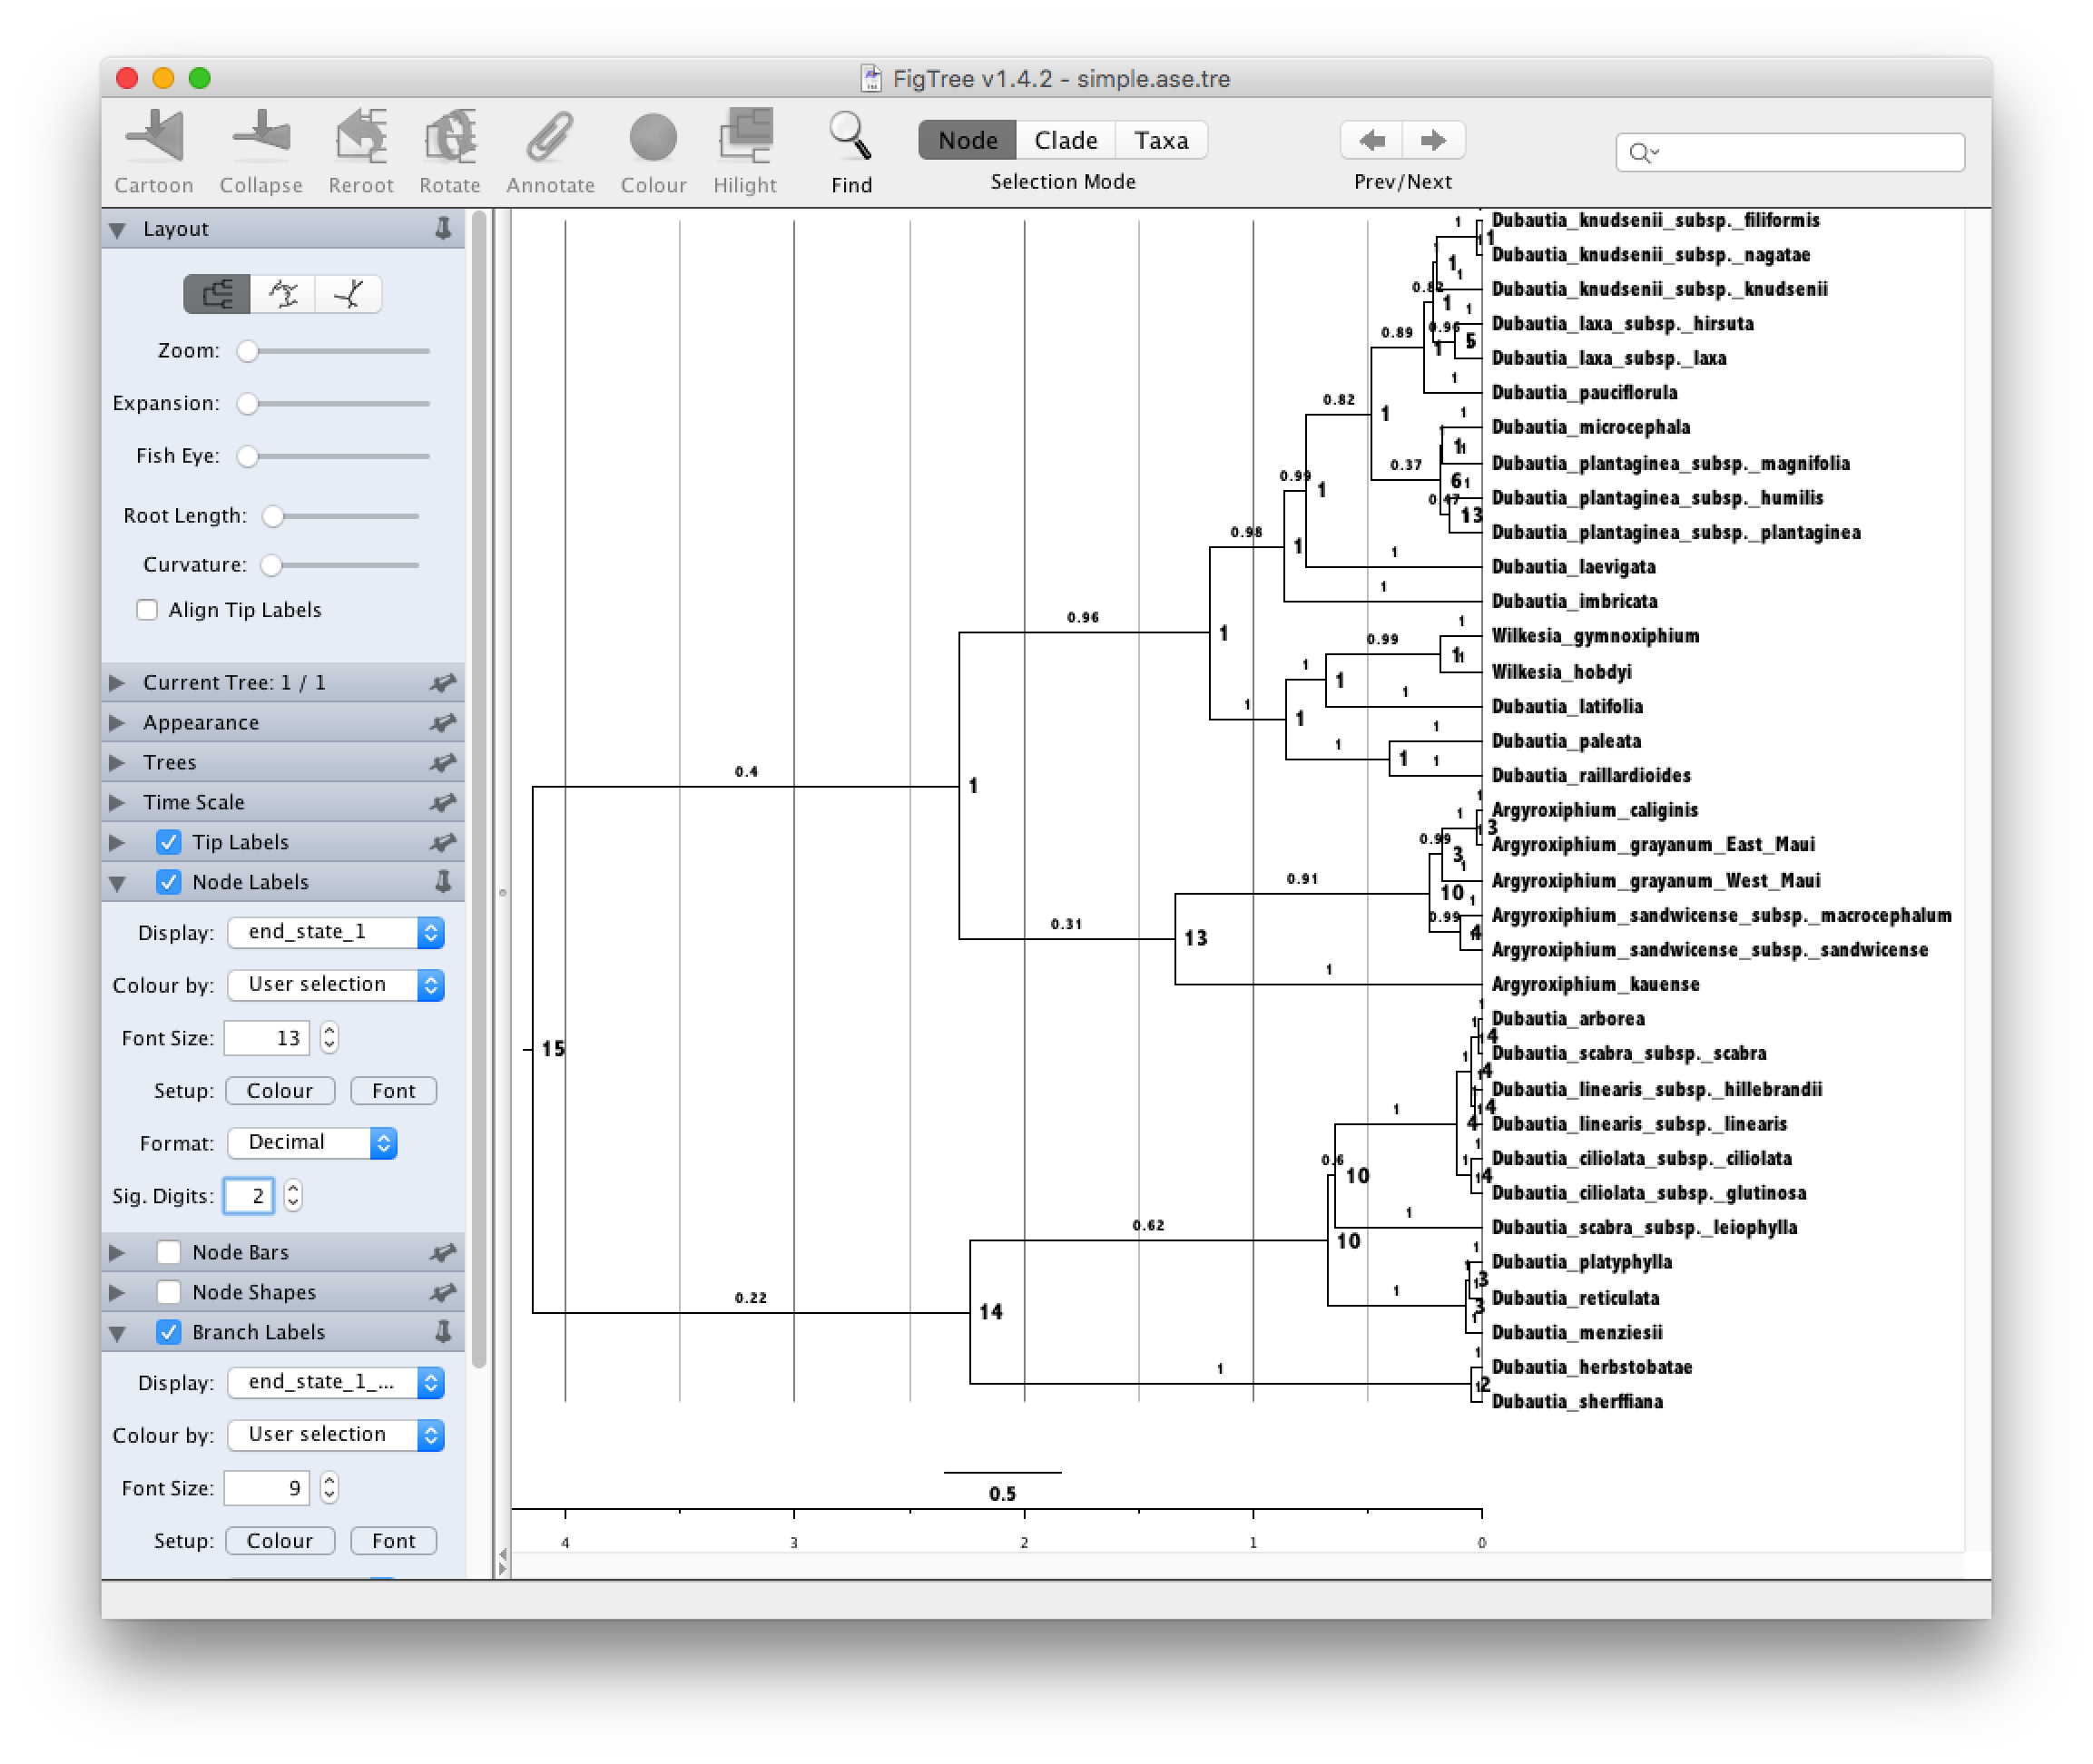
\includegraphics[width=0.6\textwidth]{figures/fig_simple_FigTree_ase.png}
\caption{Tree with ancestral state estimates. The most probable end state of each branch (before cladogenesis) is shown at each node. Branches are labeled with the posterior probability for the ancestral state on the tipwards end of the branch.}
\label{fig:simple_FigTree_ase}
\end{figure}

Nodes are annotated with the first three most probable ancestral states along with their posterior probabilities.
When the tree is a random variable, as it is in later exercises, additional information about phylogenetic uncertainty is reported.

Finally, we can also generate a figure with ancestral states in R using RevGadgets that is suitable for publication.

\begin{snugshade}
\begin{lstlisting}
# RevGadgets requires development tools for installation
install.packages("devtools")
library(devtools)

# Install RevGadgets
install_github("revbayes/RevGadgets")

# Note about ggtree dependency:
# RevGadgets requires ggtree version 1.5.14 or greater. This can be installed directly from GitHub:
install_github("GuangchuangYu/ggtree")
\end{lstlisting}
\end{snugshade}

Once this is installed you can generate a figure by executing {\tt source("plot\_anc\_state.n4.R\")} from within an R session (Fig \ref{fig:simple_RevGadgets_ase}).
Modifying the source file allows you to use the script with different datasets.

\begin{figure}[!ht]
\centering
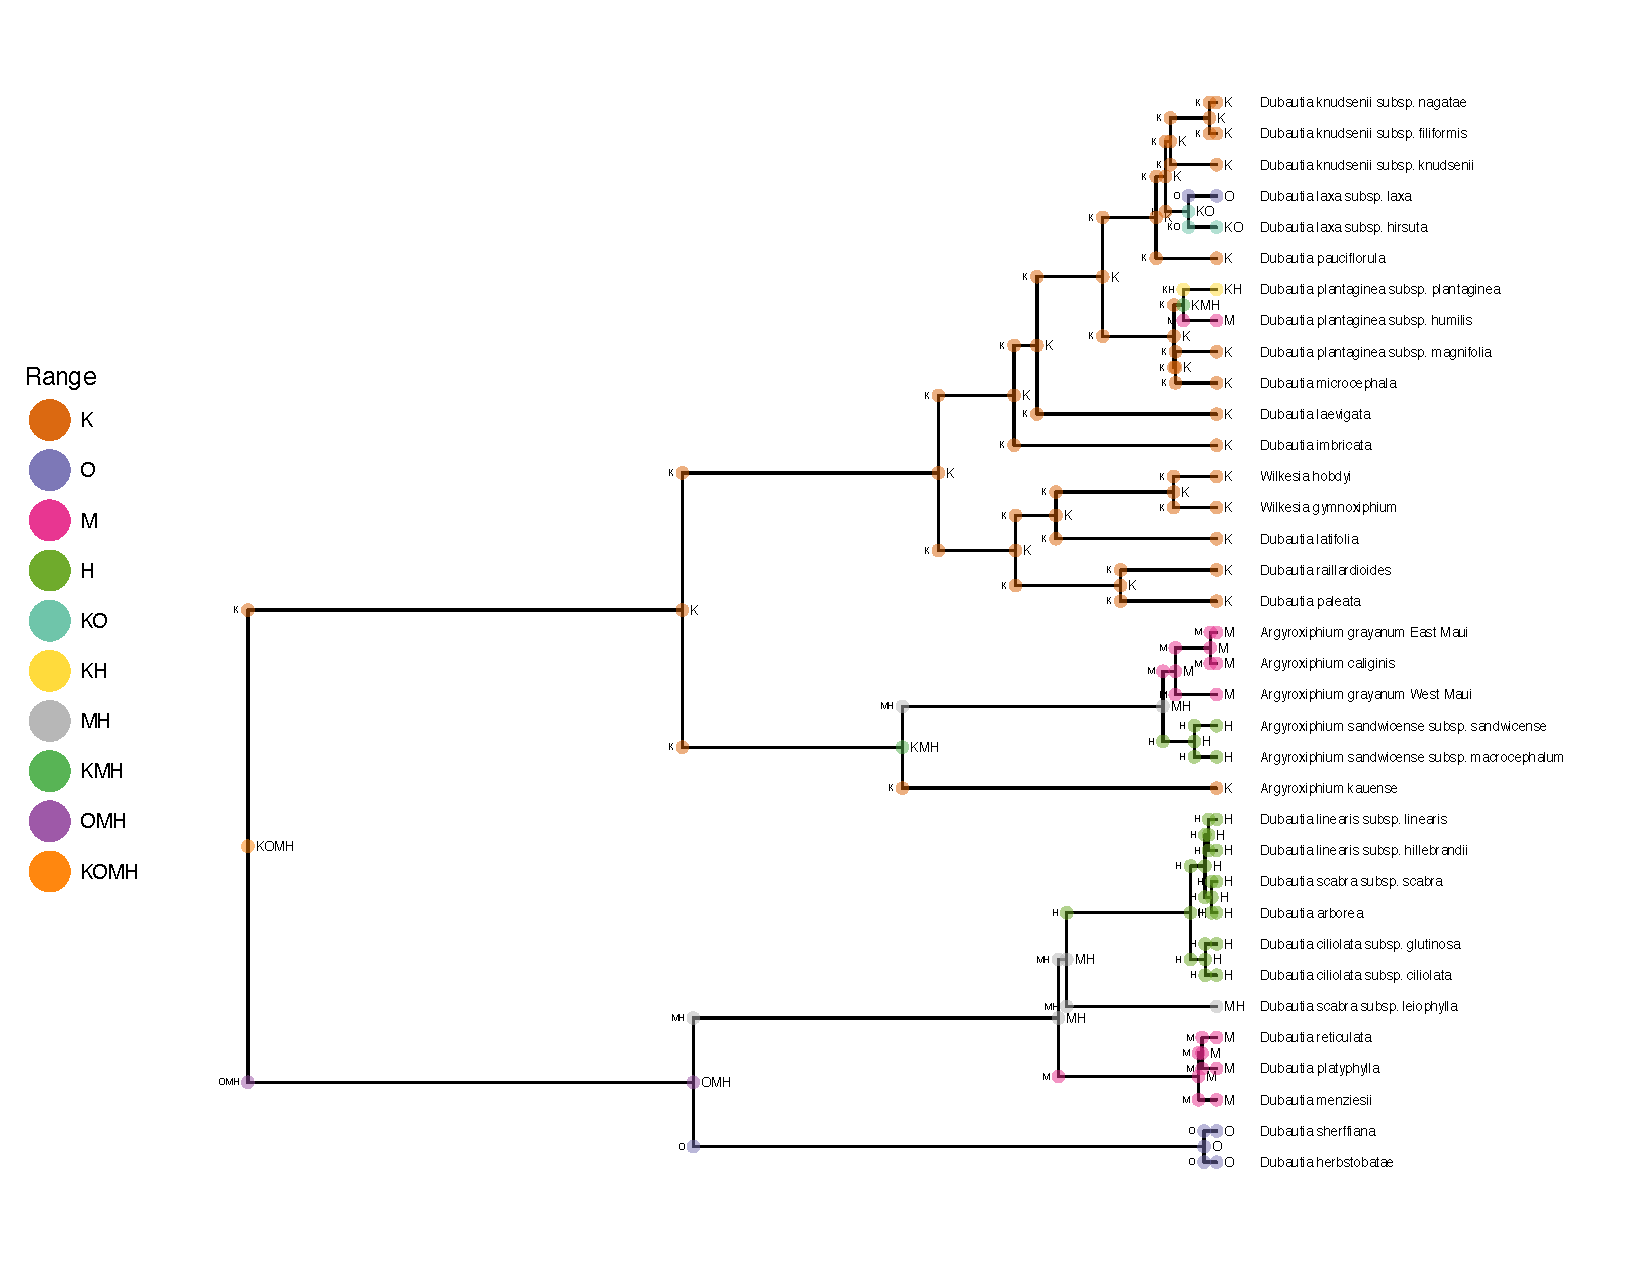
\includegraphics[width=0.7\textwidth]{figures/fig_simple_RevGadgets_ase.pdf}
\caption{Tree with ancestral state estimates for the ``simple'' analysis. Nodes are annotated with ancestral states before and after cladogenetic events. Most probable states are shown. Colors of markers indicate the range state. Sizes of markers indicate the posterior probability of that state. }
\label{fig:simple_RevGadgets_ase}
\end{figure}

Notice that the model infers a widespread ancestral range for the clade (KOMH) approximately four million years ago when only Kauai existed.
Similar geologically unrealistic widespread ranges are estimated for the Agyroxiphium clade (KMH) and the Dubautia sheriffiana+arborea clade (OMH).
The remaining tutorials will focus on improvements to the simple DEC model presented here.

\newpage
